\section{Einstufige MOS-Verstärker}

Einstufige MOS-Verstärker sind im Prinzip \textbf{Source-Schaltungen} (siehe Abschnitt \ref{Source-Schaltung}).
Diese können mit diversen Lasten betieben werden.


\subsection{Analyse von MOS-Verstärkern}

Die Analyse aller gezeigten Schlatungen erfolgt immer nach dem gleichen Schema:

\smallskip

\begin{enumerate}
    \item Arbeitspunkt mittels Grossignalanalyse bestimmen (\ref{Grosssignalanalyse / AP-Bestimmung})
    \item Kleinsignalanalyse mittels Kleinsignalersatzschaltung (\ref{Kleinsignalersatzschaltung})
    \item Verstärkung $a$ berechnen \textrightarrow\ meistens $\bm{a \approx - g_m \cdot r_{\rm out}}$
\end{enumerate}


\subsection{Widerstandslast}

Der Transistor muss im \textbf{Stromquellen-Betrieb bzw. in Sättigung} sein!

\begin{minipage}[t]{0.3\columnwidth}
    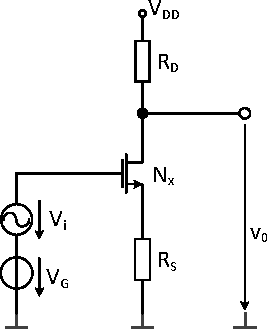
\includegraphics[width=\columnwidth, align=t]{images/07_verstaerker_mit_widerstandslast_schaltung.pdf}
\end{minipage}
\hfill
\begin{minipage}[t]{0.66\columnwidth}

    \begin{center}
        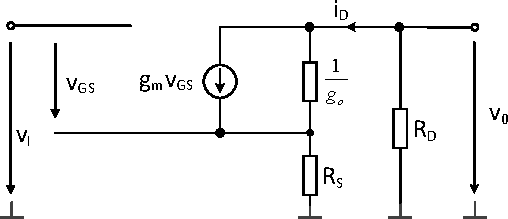
\includegraphics[width=0.85\columnwidth, align=t]{images/07_verstaerker_mit_widerstandslast_kleinsignalersatzschaltung.pdf}
    \end{center}
    
    Problem: Ein grosser Strom ist für hohe Verstärkungen wünschenswert, kostet jedoch Spannungshub.
    Die Verstärkung dieses Typs ist deshalb begrenzt auf unter 10.
\end{minipage}


\smallskip

\paragraph{Verstärkung}

\[
    a = \frac{v_{\rm out}}{v_{\rm in}} = - \frac{R_D}{R_S + \frac{1}{g_m} + \frac{g_o}{g_m}(R_D + R_S)} 
\]

\[
    \boldsymbol{ R_S = 0 \qquad  a \approx - g_m \cdot r_{\rm out} \underbrace{= - g_m (r_{\rm DS} \parallel R_D) }_{\text{Mikroelektronik}} }
\]


\paragraph{Differnetieller Ausgangswiderstand}

\vspace{-0.2cm}

\[
    r_{\rm out} = r_{\rm DS} \left( 1 + g_m R_S + \frac{R_S}{r_{\rm DS}} \right) = \frac{1}{g_o} \left( 1 + g_m R_S \right) + R_S
\]


\subsection{Diodenlast}

\begin{minipage}[t]{0.5\columnwidth}
    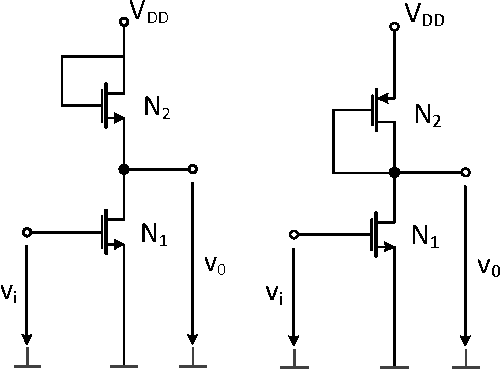
\includegraphics[width=\columnwidth, align=t]{images/07_verstaerker_mit_diodenlast.pdf}
\end{minipage}
\hfill
\begin{minipage}[t]{0.46\columnwidth}
    \paragraph{Verstärkung}

    Diode: $R_D = r_{\rm MD, N2} = \frac{1}{g_{m2}}$

    \vspace{-0.2cm}

    \[
        a \approx - g_{m1} \cdot R_D = - \frac{g_{m1}}{g_{m2}} = - \sqrt{\frac{\left( \mu C_{OX} \frac{W_1}{L_1} \right)}{\left( \mu C_{OX} \frac{W_2}{L_2} \right)}}
    \]

    \paragraph{Vorteile / Nachteile}

     \begin{itemize}
        \item[+] Spannungsabfall über Diode nicht direkt proportional zu Strom
        \item[-] N2 ist \textbf{nichtlinearer Widerstand} mit beträchtlichem Spannungsabfall
     \end{itemize}
\end{minipage}

\smallskip

\textrightarrow\ Ausgangsspannungsbereich ist weniger beeinträchtigt! \\
Diese Schaltung ist jedoch nur für keine Signalpegel und kleine Verstärkungen geeignet.


\subsection{Stromquellenlast}

\begin{minipage}[t]{0.23\columnwidth}
    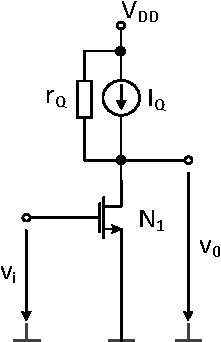
\includegraphics[width=\columnwidth, align=t]{images/07_verstaerker_mit_stromquellenlast.pdf}
\end{minipage}
\hfill
\begin{minipage}[t]{0.25\columnwidth}
    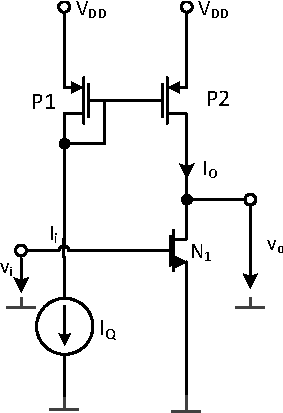
\includegraphics[width=\columnwidth, align=t]{images/07_verstaerker_mit_stromquellenlast_2.pdf}
\end{minipage}
\hfill
\begin{minipage}[t]{0.45\columnwidth}
    \paragraph{Verstärkung}

    \vspace{-0.4cm}

    \[
        a \approx - \frac{g_{m1}}{g_{o1} + g_{o2}} = -g_{m1} \cdot \left( r_{\rm DS1} \parallel r_{\rm DS2} \right)
    \]

    \paragraph{Vorteile / Nachteile}
    \raggedright

     \begin{itemize}
        \item[+] Reduzierter Spannungsabfall über Stromspiegel (nur ca. $V_\text{DS,sat}$)
        \item[+] Grosse Verstärkung wegen $r_{\rm DS2}$
        \item[-] Frequenzgang durch Miller-C zwischen Gate und Source von N1 stark beeinträchtig
     \end{itemize}
\end{minipage}

% Über den Stromspiegel fällt lediglich ca. $V_\text{DS,sat}$ ab, das Verändern des Transistorstroms beeinträchtigt den Ausgangsspannungsbereich noch weniger.
% Problem: Der Frequenzgang wird durch die Miller-Kapazität zwischen Gate und Source des Ausgangstransistors stark beeinträchtigt.


\subsection{Stromumlenkung}

\begin{minipage}[t]{0.3\columnwidth}
    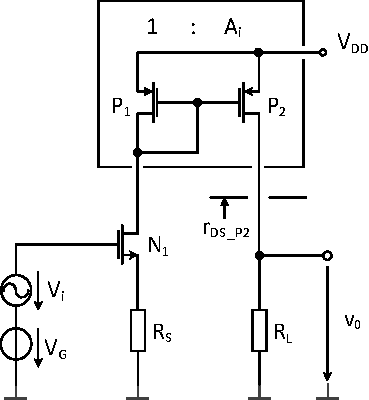
\includegraphics[width=\columnwidth, align=t]{images/07_verstaerker_mit_stromumlenkung.pdf}
\end{minipage}
\hfill
\begin{minipage}[t]{0.66\columnwidth}
    Durch den kleinen Kleinsignalwiderstand von P1 hat die erste Verstärkerstufe eine kleine Verstärkung. 
    Dadurch fällt der Miller-Effekt weniger ins Gewicht.

    \paragraph{Vorteile / Nachteile}
    \raggedright

     \begin{itemize}
        \item[+] Verbessertes Frequenzverhalten
        \item[+] Verbessertes PSR
        \item[+] Durch 1:$A_i$ einstellbare, hohe Verstärkungen
        \item[-] Zusätzlicher Biasstrom durch Ausgangszweig
        \item[-] Höhere Komplexität 
     \end{itemize}

    % Dies resultiert in
    % \begin{itemize}
    %     \item verbessertem Frequenzverhalten
    %     \item verbessertem PSR und
    %     \item durch 1:$A_i$ einstellbare, hohe Verstärkungen.
    % \end{itemize}
    % Preis dafür ist mehr Stromverbrauch sowie erhöhte Komplexität.
\end{minipage}


\subsection{Kaskode}

\begin{minipage}[t]{0.3\columnwidth}
    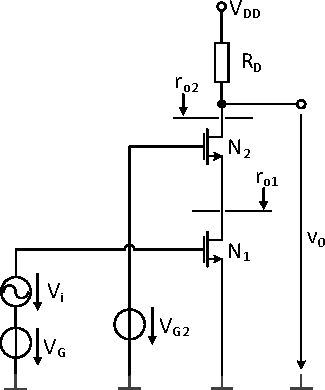
\includegraphics[width=\columnwidth, align=t]{images/07_kaskodenverstaerker.pdf}
\end{minipage}
\hfill
\begin{minipage}[t]{0.66\columnwidth}
    Durch Einsatz einer Kaskode wird eine sehr grosse Last zur Verfügung gestellt. 
    N1 bezweckt keine Spannungs-, sondern eine reine Stromverstärkung, was den Miller-Effekt pratisch völlig vermeidet.
    So hat auch dieser Verstärker ein gutes Frequenzverhalten.

    \paragraph{Vorteile / Nachteile}
    \raggedright

     \begin{itemize}
        \item[+] Sehr hoher Ausgangswiderstand $r_{o2}$
        \item[+] Hohe Bandbreite wegen kleinem Miller-C
        \item[-] Reduzierter Aussteuerbereich (wegen $G_{\rm GS2}$)
     \end{itemize}
\end{minipage}


\subsection{Wide-Swing Kaskode}

\begin{minipage}[t]{0.4\columnwidth}
    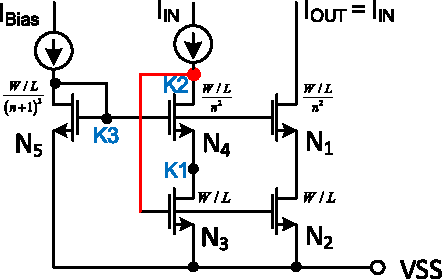
\includegraphics[width=\columnwidth, align=t]{images/07_wide_swing_kaskode.pdf}
\end{minipage}
\hfill
\begin{minipage}[t]{0.56\columnwidth}
    Durch Wählen von sehr grossen $W/L$ für die Transistoren N4 und N5 wird die minimale Ausgangsspannung $V_{\rm o, min}$ der Kaskode auf fast $V_\text{DS,sat}$ reduziert.
    
    Ausserdem kann der Arbeitspunkt mit wenig Aufwand eingestellt werden
\end{minipage}
%TODO: [Flurin] Formeln? aus V8S15
%CHECK [Simi] @ Flurin: Ich würde nicht, da diese Schaltung es nicht einmal in Zbindens Zusammenfssungs-Slide geschafft hat



\subsection{Gefaltete Kaskode}

\begin{minipage}[t]{0.68\columnwidth}
    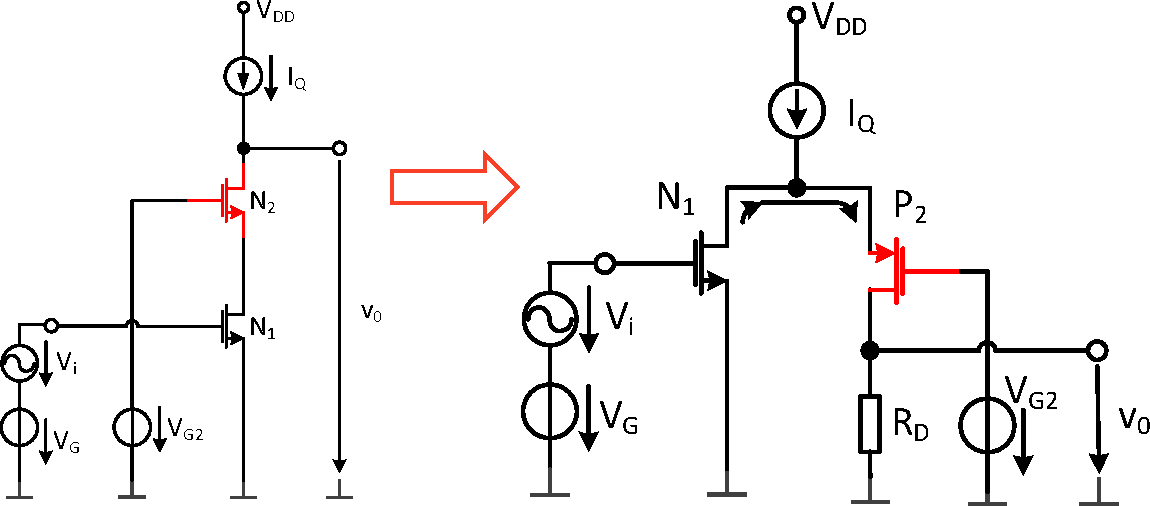
\includegraphics[width=\columnwidth, align=t]{images/07_gefaltete_kaskode.pdf}
\end{minipage}
\hfill
\begin{minipage}[t]{0.3\columnwidth}

    \paragraph{Verstärkung} %NOTE [Simi] Formel ist aus Skript

    \vspace{-0.3cm}

    \[
        a = - g_{m1} \cdot R_D
    \]

    \smallskip

    \paragraph{Vorteile / Nachteile}
    \raggedright

     \begin{itemize}
        \item[+] Hoher Aussteuerbereich
        \item[+] Sehr gute PSR
        \item[-] Zwei Strompfade\\
            (mehr Hardware)
     \end{itemize}
    % Durch 'Falten' der Kaskode kann dessen Aussteuerbereich weiter erhöht werden.
    % Dies führt auch zu sehr guter PSR, bedingt aber zwei Strompfade und so mehr Hardware.
\end{minipage}


\subsection{Verstärker mit parallelem Eingang}

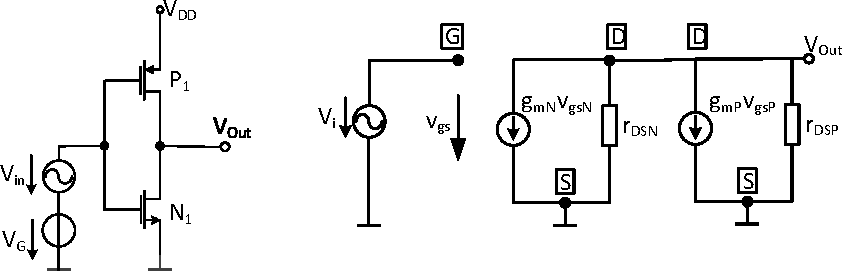
\includegraphics[width=\columnwidth, align=t]{images/07_verstaerker_mit_parallelem_eingang.pdf}

\paragraph{Verstärkung}

\vspace{-0.2cm}

\[
    a = - \frac{g_{m\_ \rm N1} + g_{m\_ \rm P1}}{g_{o\_ \rm N1} + g_{0\_ \rm P1}} = - \left( g_{m\_ \rm N1} + g_{m\_ \rm P1} \right) \cdot \left( r_{\rm DS\_N1} \parallel r_{\rm DS\_P1} \right)
\]


\paragraph{Vorteile / Nachteile}

\begin{minipage}[t]{0.48\columnwidth}
    \raggedright

    \begin{itemize}
        \item[+] Grosse Ausgangsströme und Ströme aus Last heraus möglich
        \item[+] Sehr grosse Spannungsverstärkung
    \end{itemize}
\end{minipage}
\hfill
\begin{minipage}[t]{0.48\columnwidth}
    \raggedright
    \begin{itemize}
        \item[-] Frequenzgang durch Miller-C stark eingeschränkt
    \end{itemize}
\end{minipage}

% Diese Schaltung überzeugt durch
% \begin{itemize}
%     \item grosse Ausgangsströme und
%     \item sehr grosse Spannungsverstärkung,
% \end{itemize}
% deren Frequenzgang leidet jedoch stark durch die Miller-Kapazität.

